\begin{figure}
\centering
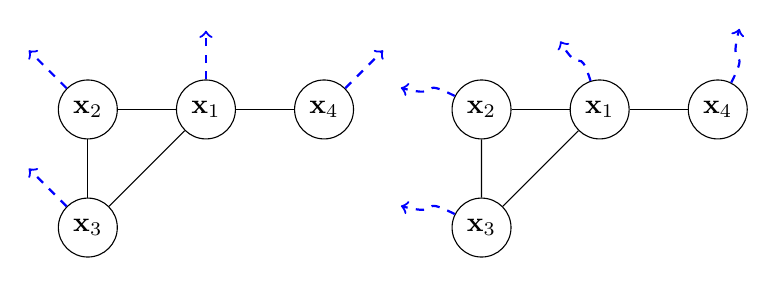
\begin{tikzpicture}
    \node[draw, circle] (x1) {$\mathbf{x}_1$};
    \node[draw, circle, left of=x1, xshift=-0.5cm] (x2) {$\mathbf{x}_2$};
    \node[draw, circle, below of=x2,  yshift=-0.5cm] (x3) {$\mathbf{x}_3$};
    \node[draw, circle, right of=x1,  xshift=0.5cm] (x4) {$\mathbf{x}_4$};
    
    \draw (x1) -- (x2);
    \draw (x1) -- (x4);
    \draw (x1) -- (x3);
    \draw (x2) -- (x3);

    \path[->] (x1) edge[out=90, in=270, looseness=2, blue, dashed, thick] ++(0,1);
    \path[->] (x2) edge[out=135, in=315, looseness=2, blue, dashed, thick] ++(-0.75,0.75);
    \path[->] (x4) edge[out=45, in=225, looseness=2, blue, dashed, thick] ++(0.75,0.75);
    \path[->] (x3) edge[out=135, in=315, looseness=2, blue, dashed, thick] ++(-0.75,0.75);

    \begin{scope}[rotate=30]
        \node[draw, circle, right of=x1, xshift=4cm] (x5) {$\mathbf{x}_1$};
        \node[draw, circle, left of=x5, xshift=-0.5cm] (x6) {$\mathbf{x}_2$};
        \node[draw, circle, below of=x6,  yshift=-0.5cm] (x7) {$\mathbf{x}_3$};
        \node[draw, circle, right of=x5,  xshift=0.5cm] (x8) {$\mathbf{x}_4$};
        
        \draw (x5) -- (x6);
        \draw (x5) -- (x8);
        \draw (x5) -- (x7);
        \draw (x6) -- (x7);
    
        \path[->] (x5) edge[out=90, in=270, looseness=2, blue, dashed, thick] ++(0,1);
        \path[->] (x6) edge[out=135, in=315, looseness=2, blue, dashed, thick] ++(-0.75,0.75);
        \path[->] (x8) edge[out=45, in=225, looseness=2, blue, dashed, thick] ++(0.75,0.75);
        \path[->] (x7) edge[out=135, in=315, looseness=2, blue, dashed, thick] ++(-0.75,0.75);
    \end{scope}
\end{tikzpicture}
\end{figure}
